%
% File coling2020.tex
%
% Contact: feiliu@cs.ucf.edu & liang.huang.sh@gmail.com
%% Based on the style files for COLING-2018, which were, in turn,
%% Based on the style files for COLING-2016, which were, in turn,
%% Based on the style files for COLING-2014, which were, in turn,
%% Based on the style files for ACL-2014, which were, in turn,
%% Based on the style files for ACL-2013, which were, in turn,
%% Based on the style files for ACL-2012, which were, in turn,
%% based on the style files for ACL-2011, which were, in turn, 
%% based on the style files for ACL-2010, which were, in turn, 
%% based on the style files for ACL-IJCNLP-2009, which were, in turn,
%% based on the style files for EACL-2009 and IJCNLP-2008...

%% Based on the style files for EACL 2006 by 
%%e.agirre@ehu.es or Sergi.Balari@uab.es
%% and that of ACL 08 by Joakim Nivre and Noah Smith

\documentclass[11pt]{article}
\usepackage{coling2020}
\usepackage{times}
\usepackage{url}
\usepackage{latexsym}
\usepackage{multirow}
\usepackage{booktabs,subcaption,amsfonts,dcolumn} 
\usepackage[T1]{fontenc}
\newcommand\nextline{\raisebox{-1.25ex}[0pt][0pt]{$\hookleftarrow$}}

\usepackage[textsize=footnotesize]{todonotes}

%\usepackage[textsize=footnotesize,disable]{todonotes}
\definecolor{Gray}{gray}{0.95}
\newcommand{\yktodo}[1]{\todo[color=green!20]{#1}}
\newcommand{\dltodo}[1]{\todo[color=yellow!20]{#1}}
\newcommand{\jttodo}[1]{\todo[color=blue!20]{#1}}
\newcommand{\corpus}{\texttt{ApposCorpus}} 

%\setlength\titlebox{5cm}
\colingfinalcopy % Uncomment this line for the final submission

% You can expand the titlebox if you need extra space
% to show all the authors. Please do not make the titlebox
% smaller than 5cm (the original size); we will check this
% in the camera-ready version and ask you to change it back.


\title{The ApposCorpus:\\ A new multilingual, multi-domain dataset for factual appositive generation}

\author{Yova Kementchedjhieva \\
  University of Copenhagen\\
  {\tt yova@di.ku.dk} \\\And
  Di Lu \\
  Dataminr, Inc.\\
  {\tt dlu@dataminr.com} \\\And
  Joel Tetreault \\
  Dataminr, Inc.\\
  {\tt jtetreault@dataminr.com}}

\date{}

\begin{document}
\maketitle
\begin{abstract}
News articles, image captions, product reviews and many other texts mention people and organizations whose name recognition could vary for different audiences. In such cases, background information about the named entities could be provided in the form of an appositive noun phrase, either written by a human or generated automatically.
We expand on the previous work in appositive generation with a new, more realistic, end-to-end definition of the task, instantiated by a dataset that spans four languages (English, Spanish, German and Polish), two entity types (person and organization) and two domains (Wikipedia and News). 
We carry out an extensive analysis of the data and the task, pointing to the various modeling challenges it poses. The results we obtain with standard language generation methods show that the task is indeed non-trivial, and leaves plenty of room for improvement.  
\end{abstract}

\section{Introduction}

\blfootnote{

    %
    % % final paper: en-uk version 
    %
     \hspace{-0.65cm}  % space normally used by the marker
     This work is licensed under a Creative Commons 
     Attribution 4.0 International Licence.
     Licence details:
     \url{http://creativecommons.org/licenses/by/4.0/}.
    % 
    % % final paper: en-us version 
    %
    % \hspace{-0.65cm}  % space normally used by the marker
    % This work is licensed under a Creative Commons 
    % Attribution 4.0 International License.
    % License details:
    % \url{http://creativecommons.org/licenses/by/4.0/}.
}

%\jttodo{note for us: I feel that we can start with a more global focus about the utlity of a system that can generate good appositives.  Useful for news reporting, summarizing information, writing assistants, etc.  and then drill down from there.  This goes for the intro and abstract.}
News articles, image captions, product reviews and many other texts mention people and organizations, whose name recognition could vary for different audiences. A piece of news, for example, may concern people and organizations that are known locally, but are not necessarily well-recognized on a global level. In such cases, news pieces targeted at a wider audience would provide background information about the entity in focus, often in the form of an \textit{appositive}. For example:
\begin{quote}
In March 2017 , Natalie Jaresko, \textit{former Minister of Finance in Ukraine}, was appointed as the board's executive director.
\end{quote}
It is unlikely that many people outside of Ukraine know the name Natalie Jaresko, so a foreign reader would likely benefit from the extra bit of information about her former occupation as justification for her new appointment. An appositive could also be less contextualized and provide information of more general importance, for example:

\begin{quote}
The conservation unit is in the Calhau bairro of São Luís, \textit{the state capital}.
\end{quote}

In general terms, appositives are phrases that appear next to a noun phrase and serve an explicative function \cite{bauer2017nominal}.
%They need not necessarily convey factual information---occasionally an appositive would also express the subjective views of the author. But as we found out, \textit{factual} appositives are ubiquitous across news articles. Collaborative writing processes could therefore greatly benefit from a system that generates such explicative phrases automatically.  
Adding such explanations to text is a multi-step process. First, one has to decide whether an entity mention needs an appositive. That may not be the case for entities that are sufficiently well-known
%for the role relevant to the given context 
or that have been introduced earlier in the text. In case an appositive is indeed needed, the next step is to choose what information about the entity to disclose. If the information is to be of a factual nature, the writer needs to have prior knowledge of the entity, or access to an external knowledge resource--\newcite{kang2019pomo} found appositives to be frequently based on facts of particular relevance to the context of the mention. Lastly, the surface form of the appositive, well-fitted to the surrounding context, needs to be produced. Viewed from the perspective of NLP, appositive generation is therefore an interesting and challenging natural language generation problem that involves reasoning over facts from an external knowledge source, with reference to a given context.

The task of appositive generation, first introduced by \newcite{kang2019pomo}, is still in its early stages and data resources are limited. %\jttodo{I like the last half of the abstract (from "we expand...")  - it clearly articulates how the task is expanded.  I vote we just copy/paraphrase it right here.} 
We expand on previous work in appositive generation with a new, more realistic, end-to-end definition of the task, instantiated by a dataset, \corpus,\footnote{Available at \url{https://yovakem.github.io/#ApposCorpus}.} that spans four languages (English, Spanish, German and Polish), two entity types (person and organization) and two domains (Wikipedia and News). While Wikipedia as a domain is curated for a world-wide audience and as such may not benefit much from appositive generation, we posit that it is a valuable source of abundant cross-lingual data which could be used as the basis for transfer learning. In addition to a large training set automatically sourced from Wikipedia, we therefore also introduce a gold standard test sourced from newswire, one of the true target domains for appositive generation \cite{kang2019pomo}. 

%The dataset allows for the study of the following research questions, previously not addressed:
%\jttodo{to come back to: we should punch up this sentence}
%\begin{itemize}
%    \item RQ1. How do NLP systems fare in the task of appositive generation in a realistic end-to-end scenario?
%    \item RQ2. How does the task difficulty vary across languages (English, German, Spanish and Polish) and named entity types (people and organizations)?
%    \item RQ3. How well do models generalize across samples and domains?
%\end{itemize}

The next section of the paper outlines the theoretical framework behind the task of appositive generation. In Section~\ref{sec:silver_data} we describe the automatic data collection procedure used to obtain training data, and in Section~\ref{sec:gold_data} we detail the further manual validation performed to obtain quality data for cross-domain evaluation. The properties of the dataset are discussed in detail in Section~\ref{sec:data_analysis}. Sections~\ref{sec:experiments},~\ref{sec:results} and \ref{sec:analysis} describe the experiments we performed and the main findings from them. Section~\ref{sec:conclusion} concludes the paper and outlines avenues for future research. 

%Recently, \cite{kang2019pomo} made the first step towards a method for the automatic generation of appositives. They introduced a dataset of appositives for \textsc{person} entities extracted from English news articles and cross-referenced with the WikiData knowledge base. Only those appositives were included in the dataset which matched a fact from WikiData. The properties of the dataset implicitly limit the task to fact selection with a guaranteed target, followed by surface-form generation. We extend the task definition to make it more comprehensive and true to real-world collaborative writing scenario. A system should firstly be capable of choosing \textit{whether or not} to generate an appositive for a particular entity. And when an appositive is indeed needed, we should not assume that the most relevant fact or facts are all present in our knowledge base. No knowledge base is complete and assuming otherwise results in a warped estimate of the system's performance in the wild.

%We introduce a dataset that corrects these limitations, covers \textsc{person} and \textsc{organization} entities (including locations), and extends to three languages in addition to English: German, Spanish and Polish. Similarly to previous work, the dataset is built automatically, and to ensure sufficient volume for all languages, it is based on Wikipedia as the main source of data. In addition to this silver standard data, we also provide a manually-annotated gold standard test set of 2000 instances per language, split equally between the two named entity types. We find that the baseline method introduced in \cite{kang2019pomo}, unsurprisingly, scores much lower when applied to our data. Further experiments show that improvements can be achieved through ..... 
%Still, results remain low due to the fact that only about 30\% of the appositives in the dataset could be successfully matched to a fact from the WikiData knowledge base, which highlights the limitations of this resource.


\section{The task: Appositive generation}
%\dltodo{I feel we should compress this whole section to make the points more straightforward. And we miss a real section for related work, such as text generation from wiki info table, cross-lingual text generation, language generation with external knowledge}
%\jttodo{I agree with Di - we should have references to that work somewhere to cover bases.  }
\label{sec:appo}
\newcite{kang2019pomo} laid the groundwork for appositive generation and our work can be seen as an expansion of their efforts. Yet, we both rename the task and redefine it in more general terms. 

\subsection{Prior work}
\newcite{kang2019pomo} introduced the task of appositive generation. To date this is the only work on this task. They designed a data collection procedure where appositives are identified by locating instances of the \texttt{appos} dependency label \cite{nivre-etal-2020-universal} in parsed text, and used it to build a dataset of appositives for \textsc{person} entities in English news articles. The candidate appositives were cross-referenced with the WikiData knowledge base \cite{10.1145/2629489} through word matching, and only those appositives were included in the final dataset which matched a fact from WikiData.
%\cite{kang2019pomo} carried out a crowdsourcing study on the level of \textit{contextualization} of appositives, and found that the best appositive for a given entity varies according to context. The main baseline \cite{kang2019pomo} experimented with is an LSTM-based encoder-decoder, which receives as input a sentence with a named entity, optionally with one preceding sentence for additional context, and a list of facts about the named entity, extracted from WikiData.  The model is augmented with an auxiliary objective, guiding the attention of the decoder towards those facts from WikiData that have a word overlap with the target appositive. 

More generally, appositive generation relates to work on joint fact selection and generation \cite{liang-etal-2009-learning,kim-mooney-2010-generative,angeli-etal-2010-simple,Konstas2013AGM}. 

\subsection{A shift in terminology}
%\dltodo{do we really need so much space to explain why we use `apposition' instead of `post-modifier'? the pomo work hasn't been a well-established shared task yet. I feel that we only need to point out that we have the similar goal with pomo work, and we name it as apposition because it describes the task more accurately.} \yktodo{I shortened the paragraph but I would prefer to keep it since it provides a decent linguistic framework for the task. As this dataset/paper has the potential to turn the task into "an established one", I want to make sure people who work on the task understand the phenomenon well enough. }
\newcite{kang2019pomo} actually called the phrases in question \textit{post-modifiers}, rather than appositives. %They do, however, explain their data collection procedure as being based on the appositive dependency label (\texttt{appos)}, so there is no doubt that they indeed built a dataset for appositive generation. 
The linguistic term \textit{post-modifier} can be seen as subsuming appositives, but it is much broader, including also prepositional, non-finite and dependent clauses that appear in postposition. Meanwhile, appositives come in two forms, nominal appositives, where a single noun identifies or qualifies another noun, e.g. President \textit{Washington}, and explicative appositives, where a pronoun, an infinitive or a noun phrase is used to explain or specify the status of a noun \cite{bauer2017nominal}. Explicative appositives are further characterized as \textit{non-essential}, meaning that they are not integral to the grammatical or semantic well-formedness of the sentence it appears in, and as such are often delimited from the rest of the sentence by punctuation marks \cite{traffis_2019}. For the purposes of providing background information about named entities, we are in particular interested in \textit{explicative appositive noun phrases}, and that is what we refer to as an \textit{appositive} throughout this work. 

\subsection{Expanding the task definition}
\label{ssec:issues}
%\jttodo{We need a short summary of what the Kang paper does either here or in the Introduction.  That they designed the task, developed a dataset and trained some models.  Otherwise the reader is still flying blind a bit on that prior work.} \yktodo{see 2.1}
%The dataset of \cite{kang2019pomo} was built by running raw text through a dependency parser and extracting noun phrases labeled as appositives and headed by a \textsc{person} named entity. In a subsequent step, each candidate appositive was word-matched against a list of known facts about its head---if a match was found with any of the facts, the candidate was added to the dataset; if not, it was discarded. The facts were drawn from the WikiData entry for the named entity in question. 
%Presumably, this fact-matching step was necessary to distinguish factual appositives from subjective ones, although the authors were not explicit about it. 
Being built with reference to WikiData, the dataset of \newcite{kang2019pomo} creates the illusion that all facts necessary to generate an appositive are available in the knowledge base. \newcite{balaraman2018recoin} studied the relative completeness of WikiData entries and found gaps to be the norm rather than an exception. Moreover, the dataset of \newcite{kang2019pomo} only includes positive samples, i.e. instances where an appositive is due. A more realistic scenario would also require the model to choose whether or not to add an appositive to a given entity mention. \corpus~ is \textit{not} constrained by WikiData in terms of fact matching, and contains positive \textit{and} negative samples, i.e. instances of empty appositives. See Figure~\ref{fig:task} for an illustration. Moreover, it is multilingual and covers both \textsc{person} and \textsc{organization} named entities. We built this dataset primarily based on text from Wikipedia, chosen for its rich cross-lingual coverage.
%\jttodo{we should mention that the dataset is English only. I really liked your slide in the talk where you laid out side by side all the ways we extend / differ from the Kang work.  Not sure if there is time or space for it now. But the paper could be improved by just spelling it out for the reader as this is a niche task.  If we don't do it here, we definitely need to for COLING}

\begin{figure}
    \centering
    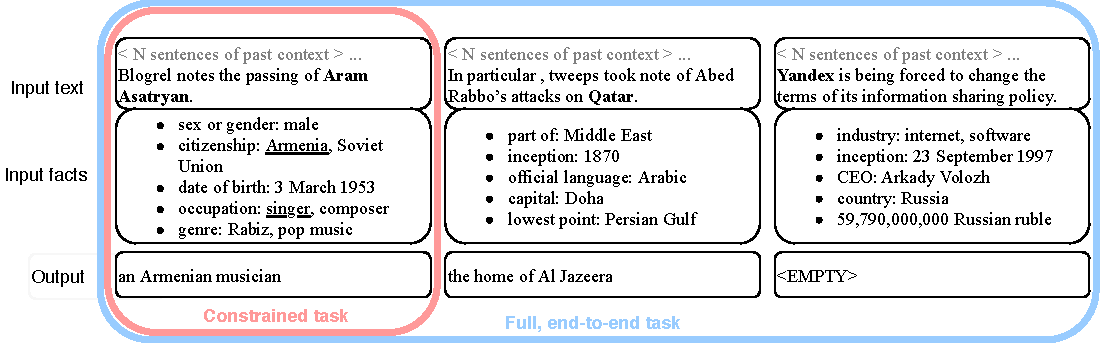
\includegraphics[width=\linewidth]{task.pdf}
    \caption{Illustration of the task in a \textit{constrained} setting, where an appositive is always due and the facts in it are always available in the knowledge base; and in a \textit{full, end-to-end} setting, where a decision has to be made as to whether or not to generate an appositive, and the facts in the appositive may be missing from the knowledge base. The entity in focus is shown in bold, the relevant facts are underlined (where available), and the $<$EMPTY$>$ tag means no appositive is needed. Optionally, previous context can be included in the input, e.g. the three previous sentences--this is not shown in the figure.}
    \label{fig:task}
\end{figure}

%Moreover, the dataset is biased towards the kind of facts that are likely to be listed on WikiData. 
%As we report later on, another artifact of the procedure concerns target length: on average, the length of appositives that yield a non-zero match with WikiData facts is twice as high as the length of all appositives in our data. This is not surprising, as greater length provide more opportunity for a word overlap, but it is undesirable to have such biases in the data. 
%\jttodo{to come back to: a compact list of all the task/dataset expansions}
%\jttodo{can we have a segue paragraph here that sets up the Silver and Gold dataset collections - specifically, why we are doing them.  }


\section{Dataset collection: Wikipedia}
\label{sec:silver_data}
%\dltodo{reviewers may argue that it's easy to crawl Spanish/German news online. and we also have a gold dataset based on news corpora in next section. it seems the main reason to use wikipedia is we can have silver standard annotation automatically, rather than availability of the news corpora} 
%Wikipedia is designed to contain text exclusively of a factual nature and as such is perfectly fit as a \textit{main} source of data for the task of \textit{factual} appositive generation. 
We used the March 2020 Wikipedia dump\footnote{\url{https://dumps.wikimedia.org/}} for English, Spanish, German and Polish, which we parsed with WikiExtractor,\footnote{\url{https://github.com/attardi/wikiextractor}} preserving internal links.\footnote{These links point to other pages on Wikipedia and allow us to identify the Wikidata entry for the given named entity.} The choice of these particular languages was mostly based on the availability of good dependency parsers. Since dependency parsing is an integral step of the data collection process \cite{kang2019pomo}, it has to be as precise as possible, to maximize the quality of the outcome.\footnote{We only considered parsers with labeled accuracy score over $90.0$}  Below, we describe in detail the data collection procedure. 

\subsection{Preprocessing}
We processed every article as follows: 
%\dltodo{maybe better to switch the order of tokenize and segment}\yktodo{Not sure, the order in which these are performed is actually tokenization first, segmentation second}
(1) tokenize the text and segment sentences; %\dltodo{what is internal link exactly?}
(2) normalize mentions of the entity in the article's title and annotate them with internal links; (3) identify sentences which contain a linked named entity listed as an instance of type \textit{human} or of (a subclass of) type \textit{organization} in WikiData (corresponding to the \textsc{person} and \textsc{organization} named entity types); 
%\dltodo{do you mention the performances of the parser for those languages in the paper?} \yktodo{I now added a footnote abote about performance threshold}
(4) run a dependency parser 
%\jttodo{Kang et al. just use a regular English-focused dependency parser and not UD right?  We should make it clear somewhere in Sec 3 (probably here) that we use a UD parser and the reason (enables consistent, multilingual processing or something like that)} \yktodo{Kang et al use Stanford CoreNLP which is also based on the UD schema} 
on these sentences. 
Steps (1) and (4) were performed with Stanza \cite{qi2020stanza}.

\subsection{Detecting  appositives}
Any instance of the \texttt{appos} label that depends on a linked named entity and is separated from it with a comma or an opening parenthesis was considered a valid candidate. In this case, we recorded the source sentence, replacing the appositive with special token \texttt{<appos>}, as input data, and the appositive as a target. The beginning of the appositive was taken to be the first token after the comma or opening parenthesis, and the end is taken to be the last token before the next comma/semicolon/full stop (if beginning was marked by a comma) or closing parenthesis (if beginning was marked by an opening parenthesis). We discarded any commas and parenthesis surrounding the appositive, but kept semicolons and full stops as part of the input sentence. We also recorded the three preceding sentences from the article and one following sentence.
%\jttodo{did we actually use the three preceding sentences?} 
%\yktodo{we tried 0, 1 and 3 and results were not definitively in favour of either one. I'll say that in the results} 
Similarly to \newcite{kang2019pomo}, we process one appositive per sentence, i.e. if there are multiple appositives in a sentence, we select the first one and do not consider the rest.

Appositives containing just dates (usually the date of birth and/or death of a person) are ubiquitous across Wikipedia articles to the point that they constitute up to 30\% of the data samples that we get with the procedure described above. 
%This imbalance in the data is a particularity of the encyclopedic domain, which could lead to a major bias in a more general context. 
%Moreover, this information is always presented in a very formulaic way, so it does not pose a challenge from a natural language generation point of view.
We reduced this imbalance in the data by downsampling this type of appositives to only 10\% of its occurrences. 

\subsection{Negative samples}

We added negative samples to the dataset, matching the number of positive ones. They were drawn according to the following criteria: (1) there is a \textsc{person} or \textsc{organization} entity in the sentence, (2) it is not followed by a comma or opening parenthesis, and (3) the rest of the sentence does not contain an appositive dependent on the \textsc{person} or \textsc{organization} entity. Condition (2) was used to reduce the chance of including instances of appositives that were not correctly tagged as such by the parser (recall that appositives are often delimited from the rest of the sentence by a punctuation), while (3) was used to ensure that we did not include instances that contain a non-essential appositive, which the author had failed to delimit by any punctuation. In negative samples the input is the original source sentence with an added token \texttt{<appos>} just after the \textsc{person}/\textsc{organization} entity, and the target is a special \texttt{<EMPTY>} token. 

%\subsection{Quality control}
%Since our dataset was created automatically, some of the positive instances in it are not actually appositives. We manually inspected 100 random positive samples from each subset of the data, marking as invalid any instance where the target was either incomplete (i.e. it spans part of an appositive but not the full appositive), overcomplete (i.e. spans text beyond the end of the appositive), or not at all an appositive. The percentage of invalid instances, or noise, was found to vary greatly: from 6\% for \textsc{person} appositives in German to 27\% for \textsc{organization} entities in Spanish (see row \textit{Noise} in Table~\ref{tab:silver_data_stats}). 
%\jttodo{I'll be argumentative here: does this mean that all of our silver evaluations are unreliable?  That is one inference a reader could do with that sentence} \yktodo{Honestly, I do believe that do be the case, but its certainly a consideration many other papers, including Kang et al. disregard.} 

%The automatic data collection procedure described above could be expected to yield a certain level of noise. While this is acceptable for training purposes, evaluation stability may suffer in a noisy setting. For this reason, the quality of the News test set we developed was manually validated, i.e. it is gold standard. 

The procedure described above was used to collect \textit{training} data for factual appositive generation. As it is our goal to study the potential of a cross-domain approach to appositive generation, the \corpus~also contains an out-of-domain test set, sourced from newswire. 

%\subsection{Identifying candidate appositives}
%We use a small set of heuristics to identify postmodifiers in Wikipedia articles, based on punctuation and word matching. Postmodifiers are often demarcated by commas or brackets. We only consider languages for which we know this to be the case. Once we identify a potential candidate by matching the pattern $$\langle{person}\rangle{}\langle{comma/LRB}\rangle{}\langle{text}\rangle{}\langle{comma/RRB}\rangle{}$$ we check whether there is a word overlap between the matched $text$ and any facts we have extracted from WikiData about the respective $person$. We exclude stopwords from consideration when measuring word overlap and consider any overlap $>1$ to mean that the $text$ carries factual information about the $person$. Through manual analysis of the results obtained with this method, we compile a further list of rules, for better filtering of the candidates. We found that the main type of non-appositive that makes it past our heuristics are postmodifiers, of the prepositional and relative clause types, so we discard any candidates which start with a preposition or a relative pronoun (e.g. \textit{who, whose, that} etc.) We further find that discarding candidates which start with any stopword is more beneficial to the precision of the method than it is detrimental to its recall. Wikipedia articles use the comma-comma or LRB-RRB pattern heavily for date of birth and death information; we discard these candidates, as they don't classify as appositives.
%based on number matching and matching of the symbols often used to mean birth and death (asterisk and a cross symbol). 
%Lastly, the pattern we use can match lists of people, where the $text$ which comes after $\langle{person}\rangle{}\langle{comma/LRB}\rangle{}$ is just another name. We filter out such cases based on capitalization: a candidate cannot start with a capital letter. This rule is problematic for German, where all nouns are capitalized, and for languages like Arabic and Chinese, where no case distinction is made, so there we instead check that the first word of the candidate cannot be found in list of people we've extracted from WikiData. For other languages, we find the more general case-based rule to again benefit precision more than it hurts recall. 

\section{Dataset collection: News}
\label{sec:gold_data}

We sourced our data for cross-domain evaluation from the news domain, following previous work \cite{kang2019pomo}, using these news corpora: Global Voices (English, Spanish, German, Polish) \cite{TIEDEMANN12.463}, News Commentary (English, Spanish, German) \cite{TIEDEMANN12.463} and Paralela \cite{pkezik2016exploring}.  %Based on the observations concerning noise levels in the automatically processed Wikipedia data, we deemed it necessary to manually validate the quality of this news-based test set, to ensure evaluation stability. 

%\jttodo{in the prior sections we used subsections...should we do that here instead of paragraph to make it consistent? }

%\dltodo{reviewers may ask why don't you use some open tools for entity linking}
\subsection{Entity linking} Unlike Wikipedia, where entities are explicitly linked to WikiData entries through internal links, here, we had to perform additional entity linking. We did so in the following manner: (1) extract candidates from WikiData based on exact match between the full span of the named entity and all aliases of entities in the respective subset of WikiData (instances of type \textit{human} if NER label is \textsc{person} , else \textit{organization}), (2) obtain relative alias frequency distributions from Wikipedia, and (3) the candidate entity with the highest relative frequency given the alias is selected. We chose to use this prior-based method instead of a modeling approach since off-the-shelf entity linkers were not available for all the languages involved. 
Candidate appositives were then identified as described in 3.2. 

As errors could occur both in the entity linking and in the appositive detection, we hired manual annotators to verify the output of the two procedures (see details in Appendix~\ref{manual}). The News portion of the \corpus~ is therefore gold standard and will serve for stable, accurate evaluation. 

\subsection{Negative samples} We added $1,000-n$ negative samples to each subset of the data, where $n$ is the number of positive samples.
%(listed in row \textit{Pos} in Table~\ref{tab:gold_data_stats}). 
The exact ratio of positive samples in each test set is reflected in the \texttt{always yes} baseline shown in the Results section (see Figure~\ref{fig:gold}a), a dummy baseline which always predicts an appositive. 
%\jttodo{this popped in my head: couldn't we use these numbers in Fig 1b to serve as a baseline?  (do the majority class). Basically, what is the F1 if you just try and predict the majority class for every instance (in whether an appos is needed or not) }
%We also report WikiData coverage, which is similar to that observed for the silver data for all English, Spanish and German, and it substantially lower for Polish \textsc{person} appositives.    

\section{Data analysis}
\label{sec:data_analysis}
This section outlines some findings on the properties of our dataset, based on general statistics and WikiData cross-referencing. The procedure described above yielded less than four thousand samples of \textsc{org} appositives for Polish, so this subset is omitted from the \corpus. 

\begin{table}
    \small
    \begin{subtable}[l]{0.5\textwidth}
    \centering
    \begin{tabular}{clllll}
          && en & es & de & pl \\
          \hline
         %\multirow{3}{*}{\textsc{per}} & size &  558,990 & 163,788 & 269,204 & 13,880 \\
         \multirow{4}{*}{\rotatebox{90}{\textsc{per}}} & Size &  559k & 164k & 269k & 14k \\
         %& Pos & 279.5k & 82k & 134.5k & 7k\\ 
         &Length&3.4&4.16&2.7&2.67\\
         %& noise (\%) & 17  & 12 & 6 & 18  \\
         & WD (\%) & 25.5 & 28.1& 21.2 & 22.3\\
         \hline
         \multirow{4}{*}{\rotatebox{90}{\textsc{org}}} & size & 612k & 104k & 333k & -\\%7k \\
         %&Pos&306k&52k&166.5k&-\\
         &Length&2.19&4.09&1.64&-\\%2.53\\
         %& noise (\%) & 26 & 27 & 13 & - \\%58\\
         & WD (\%) & 27.8 & 24.9& 22.2 & -\\%27.0\\
    \end{tabular}
    \caption{Wikipedia data}
    \label{tab:silver_data_stats}
    \end{subtable}
    \begin{subtable}[l]{0.5\textwidth}
    \centering
    \begin{tabular}{clllll}
          && en & es & de & pl \\
          \hline
         \multirow{4}{*}{\rotatebox{90}{\textsc{per}}} & size &  1k & 1k & 1k & 1k\\
         %& Pos & 500 & 482 & 544 & 439 \\
         & Length & 4.07&3.51&3.43&2.32\\
         & WD (\%) & 29.3& 30.8 & 21.7 & 20.7 \\
         \hline
         \multirow{4}{*}{\rotatebox{90}{\textsc{org}}} & Size &  1k & 1k & 1k & -\\
         %& Pos & 499 & 402 & 456 & -\\
         & Length & 3.31 & 3.08 & 1.87 & - \\
         & WD (\%) & 35.4& 30.0& 22.8 & -  \\
    \end{tabular}
    \caption{News data}
    \label{tab:gold_data_stats}
    \end{subtable}
    \caption{Dataset statistics. \textit{Size}: full dataset size, \textit{Length}: average appositive length, \textit{WD}: ratio of appositives matching a fact from WikiData.}
    \label{tab:data_stats}
\end{table}

\subsection{General statistics}
%\dltodo{i think we should include more examples at lease in appendix} \yktodo{examples of what, Di?}
Table~\ref{tab:data_stats} lists some statistics about the two parts of the dataset, one based on Wikipedia (\textit{Wikipedia data}) and the other on news (\textit{News data}). Row \textit{Size} refers to the full size of the data as split into language and entity type. We further split each Wikipedia subset for training (70\%), validation (15\%) and testing (15\%).  
%for training, validation and testing. 
Size varies greatly across the data, with the Polish \textsc{person} subset being merely 2.5\% the size of the English \textsc{person} subset. This relates both to a difference in the Wikipedia sizes for these languages  (6M English articles v. 1.4M Polish articles) and to a difference in the frequency of use of appositives across the languages.  

Row \textit{Length} in Table~\ref{tab:data_stats} lists the average number of tokens per appositive, which varies from two to four tokens, and is generally lower for \textsc{organization} appositives than for \textsc{person} ones. 

\subsection{Cross-referencing with WikiData}

As discussed before, fact matching is not part of our data collection procedure, but at training time it would be beneficial to have access to a knowledge base such as WikiData, and to draw from it, when possible. So we extract the WikiData entries for all named entities in our dataset and perform word matching between facts and appositives in the following way: (1) tokenize the fact and the appositive, (2) remove stopwords, (3) measure token overlap. If the overlap is non-zero, we consider there to be a match and annotate the fact as \texttt{used}.\footnote{We experimented with other thresholds (2 and 3-word overlap) and with fuzzy matching, but found this method to work best.}
%If no fact is found to be matching the appositive, all facts are marked as \texttt{false}, and we add one more item to the list of fact, \textit{None of the above}, marked as \texttt{true}. 

Cross-referencing the data with WikiData is also useful as an insight into the makeup of the data, albeit an insight that is biased the scope and completeness of the knowledge base.


\paragraph{Coverage} Row \textit{WD} %\jttodo{what does WD stand for really? } \yktodo{WikiData. Maybe we could reword the caption of Table1 to make that more clear} 
in Table~\ref{tab:silver_data_stats} shows the rather low percentage of appositives from the Wikipedia dataset that are matched to at least one fact from WikiData: from 21.2 for German \textsc{person} appositives to 28.1 for Spanish \textsc{person} appositives. The numbers for the News test set, shown in Table~\ref{tab:gold_data_stats}, are mostly similar to those for the WikiData. Another way to view these percentages is as an effective upper bound on the performance of a model trained with WikiData as the source of knowledge. Further work in identifying other sources of facts for appositive generation and new means of integrating them into a model could therefore prove very fruitful. 
%\jttodo{do we actually do this comparison?  What if we use the WikiData as an oracle, what do F-score / BLEU / Meteor scores look like?  Because we can't compare percentages to those scores to figure out the upper bound.  I think this would be great to do and give a better explanation for the low automatic numbers.  COLING?}
%\jttodo{can you add some text detailing what this means for a real-world evaluation?  basically, this serves as an upper-bound of sorts.  It may not be likely to get over 35.9\% with a model that solely uses Wiki as its source of facts about the world.  Something like that?  }


We manually inspected a random sample of 100 appositives from the English section of the Wikipedia dataset that were not matched to any fact from WikiData. In the majority of cases, the appositives concerned the occupation of a person, their position within an organization, their country of origin, or other type of information that is typically found in WikiData, but was missing for the given named entry.

%In a few cases, however, we deem the underlying information to be of a kind that is rarely found in WikiData to begin with: one instance was a statistic from a (regular) sports game: ``Chad Jenkins (\textit{3.2 innings pitched})''; another concerned friendship: ``Alvin Tonry, \textit{close friend of Bussie}''---the only properties that come up as related to the word \textit{friend} in WikiData are \textit{unmarried partner, significant person} and \textit{false friend}, i.e. friendships as such is not part of the ontology; another entity type we did not observe in the Wikipedia data, but was frequent in the news corpora is Twitter handles, also not present in the WikiData ontology.

%In a handful of cases, the underlying information does actually appear in the WikiData entry, but was not correctly matched to the appositive due to different phrasing, or because it is a generalization or qualification. Consider the phrase ``Muzio Clementi, \textit{a renowned teacher}''. The WikiData entry for Muzio Clementi states that he was \textit{a music pedagogue}, a.k.a. \textit{teacher}, and lists a number of sources in which he was described, from which one could deduce that he was indeed \textit{renowned}. 
%This last subset of appositives, falsely perceived as not matching any WikiData facts, is particularly interesting as it could be revealing about the ability of an appositive generation system to paraphrase and generalize, rather than just copy a fact with minor changes. 
%\jttodo{if we need space, it's possible to trim the prior three paragraphs down without loss of meaning }

\paragraph{Composition} We studied the composition of the data, as observed with reference to WikiData. We performed our analysis on all languages and found that similar trends hold cross-lingually, so here we discuss the English portion of the data only, and in the Appendix~\ref{composition} we include the corresponding tables for Spanish, German and Polish. %\jttodo{I'm not sure what the goal of this subsection is. Let's get clarity at the meeting.}

%There are two named entity types contained in the data, \textsc{person} and \textsc{organization}, the two categories based on the WikiData instance types \textit{human} and \textit{organizations}. While the former is a homogenous category, the latter spans a range of entity subtypes. The top ten entity subtypes in this category found  in the main dataset and the news dataset are listed in Table~\ref{tab:wikidata}, section \textsc{ORG-ENTITY}. Subtypes on the News data side that are not found on the Wiki data side are colored in grey. Notice the high overlap between the compositions of two datasets in terms of entity types.

We looked at the types of facts that were matched to appositives from the News data. For all fact types that constitute 3\% or more of all facts matched, we also looked at their frequency in the Wikipedia data. Results are shown in Table~\ref{tab:wikidata}. We see that half of the top fact types in the News dataset are also well-attested in the Wikipedia data, i.e. their relative frequency is 3\% or more. We can expect that knowledge concerning appositives based on these fact types would trivially transfer from one domain to the other. The low frequency for the remaining fact types (cf. \textit{has quality} and \textit{capital of}), on the other hand, poses a challenge whose solution would require deeper natural language understanding and, possibly, explicit domain transfer techniques.   

\begin{table}[]
    \centering
    \small
    \begin{tabular}{clllclll}
                         &Fact type&News (\%)&Wiki(\%)&&Fact type&News (\%)&Wiki(\%)\\
                         \hline                         %\multirow{10}{*}{\rotatebox{90}{\textsc{org-entity}}}&sovereign state&sovereign state\\
                         %&country&country\\
                         %&business&business\\
                         %&organization&big city\\
                         %&big city&\textcolor{gray}{enterprise}\\
                         %&political party&city\\
                         %&city&city 1000000+\\
                         %&city of the USA&political party\\
                         %&city 1000000+&\textcolor{gray}{capital}\\
                         %&university&\textcolor{gray}{landlocked country}\\
                         %\hline                         
                         \multirow{7}{*}{\rotatebox{90}{\textsc{per}}}&  position held & 20.9 & 9.4 & \multirow{7}{*}{\rotatebox{90}{\textsc{org}}} & instance of&23.1&10.9\\
                          & occupation&15.9&10.6&& official website & 6.3&6.2\\
                          & citizenship&10.1&4.3 && country&5.9&3.3\\
                          & member of party&7.6&1.9&& member of&4.2&2.4\\
                          & award received&5.2&3.9&& subsidiary&3.5&2.1\\
                          & nominated for&3.6&0.4&& capital of&3.2&0.1\\
                          & educated at&3.1&3.1&& has quality&3.0&0.0\\
                         \hline
                         
                         
                        
                         
                         
                         
                         
    \end{tabular}
    \caption{Top fact types. English. }
    \label{tab:wikidata}
\end{table}

\section{Experiments}
\label{sec:experiments}

%\jttodo{Can you add some segue sentences here or at the end of Section 5 where we give a quick overview of what we want to accomplish with models, and how this differs from Kang.  Because we try some new things and it is important we get that across}

To show how the new task formulation can be used,  
we experiment with three established language generation methods: the main method of \newcite{kang2019pomo}, which we refer to as \texttt{base}; an extension of \texttt{base}  with external knowledge injected through embeddings with knowledge-base grounding (\texttt{KB}); and a model enhanced with an explicit copy mechanism (\texttt{copynet}, \newcite{gu-etal-2016-incorporating}). Notice that our goal here is not to build the best model for this task, but to develop reasonable models which can serve as baselines for future work in this area.\footnote{We also experimented with a transformer architecture, but encountered optimization problems. See details in Appendix~\ref{transformer}.}

%\dltodo{what is the definition of F1 score here?which BLEU? 1,2,3, or 4?}

\subsection{Architectures}
%\jttodo{For each of the models below, write their abbreviated name in the paragraph heading.  (base, kb, copynet) so it is easy to link}
\paragraph{LSTM baseline, \texttt{base}}
\newcite{kang2019pomo} introduced an LSTM-based encoder-decoder architecture with an auxiliary objective used to guide the attention of the decoder towards the WikiData facts that were matched during the data collection process. Input sentences and facts are represented with the same word embeddings and encoded by separate biLSTMs. The decoder is initialized with the encoding of the input and attends over the encodings of the facts. Our only modification here is to add a ``None of the above'' item to the list of facts about an entity and point the attention to that when no other fact was matched or the appositive was empty (i.e. for negative data instances).

\paragraph{LSTM with external knowledge, \texttt{KB}}
External knowledge can be beneficial to a better understanding of the context and how it relates to the different facts known about an entity. Here, we use the same architecture as above, but initialize the embedding matrix of the model with the NTEE (Neural Text-Entity Encoder) word embeddings,
%\jttodo{explain what the NTEE word embeddings are} 
trained on Wikipedia with WikiData grounding \cite{yamada-etal-2017-learning}. They aim to represent a text and its relevant entities close to each other. We deem these embeddings suitable for our modeling setup, where input text and facts are represented in a shared space. Unfortunately, the NTEE embeddings are available only for English. So we used word-level translation to ``project'' them to Spanish, German and Polish. See more details in Appendix~\ref{projection}.    This approach is likely to introduce some noise, but we only use the projection to initialize the embedding matrix which is then further trained. So any signal coming from the embeddings can be used by the model and any noise can be filtered out during training. 

\paragraph{LSTM with a copy mechanism,  \texttt{copynet}}
%As reported in Table~\ref{tab:data_stats}, word overlap was observed between WikiData facts and appositives around 25\% of the time for most languages and entity types. Motivated by this observation, 
Motivated by the observation that there is an overlap of at least one token between WikiData facts and appositives for about 25\% of the datapoints in our dataset, we experiment with a method that allows the decoder to copy tokens directly from the input: Copynet \cite{gu-etal-2016-incorporating}. \newcite{kang2019pomo} correctly point out that in their constrained data setting, where data points were selected based on word overlap with WikiData facts, using a copy mechanism would result in double-counting, i.e. artificially boosted results. In our data setting, however, this is not the case.
\\

All three approaches are  end-to-end in the sense that we do not split up the classification task of whether or not to predict an appositive from the task of generating an appositive where it is due. As negative samples in the dataset have the special \texttt{<EMPTY>} token as target, the models are performing the classification task \textit{implicitly} by choosing whether to predict the \texttt{<EMPTY>} token or not.

Preliminary experiments with the \texttt{base}  architecture showed that the choice between providing the model with three sentences of preceding context, one or zero had little impact on its performance, so all results reported below use one sentence of preceding context, following \newcite{kang2019pomo}. Further details on the implementations and the hyperparameters we used can be found in Appendix~\ref{implementation}. 

\subsection{Evaluation}
We follow \newcite{kang2019pomo} in the choice of performance metrics for predictions over the positive instances in the data: we measure F1 score of the predicted bag-of-words excluding stopwords; BLEU \cite{10.3115/1073083.1073135} over n-grams, where $n=1,2,3$;\footnote{\newcite{kang2019pomo} also included four-grams, but seeing that the average length of an appositive across the different subsets of the data is 3.08 tokens, we exclude four-grams from consideration.} and METEOR \cite{denkowski-lavie-2014-meteor}, which supports stemming and synonymy only in English, Spanish and German, so these features are not used for Polish. We use accuracy to measure the models' ability to determine when an appositive is due. 
%We chose to report precision and recall for the latter as well, as the trade-off between these values proved relevant to the analysis of the models' performance.

\section{Results}
\label{sec:results}

\begin{table}
    \centering
    \small
    \begin{tabular}{cllllll}
         Train setting&Test setting&Dataset&Acc(\%)&F1 & BLEU & MET. \\ 
         \hline
         \multirow{2}{*}{constrained}&
         \multirow{2}{*}{constrained}& ApposCorpus (News) & - & 19.61	&7.93	&9.12 \\
         && PoMo & - &  11.21&	3.44&	5.03 \vspace{1mm}\\
         \multirow{4}{*}{end-to-end}&\multirow{2}{*}{constrained}& ApposCorpus (News) & 95.0 & 10.76 & 3.39 & 4.41 \\
         &&PoMo&91.7 & 4.52	&0.57	&2.03\vspace{1mm}\\ 
         &end-to-end&ApposCorpus (News) &72.33 & 5.97 & 1.03 & 2.96\\

         %&&base$^{PoMo}$ & - & 35.2 & 13.7 & 15.3\vspace{2mm}\\ 
    \end{tabular}
    \caption{Generation of English \textsc{person} appositives in a constrained v. end-to-end train and test setting.}
    \label{tab:RQ1}
\end{table}

We view the results of our experiments from two angles: one concerns the expansion of the task definition we achieve with \corpus, from a constrained scenario to an end-to-end one; the other concerns the increased coverage of the dataset, which allows us to compare and contrast appositive generation across different languages and named entity types. 

\subsection{Constrained v. end-to-end scenario}
%\jttodo{I found 6.2 a little hard to follow.  There are all these settings to keep track of.   I'd have to spend more time on it to give more actionable feedback so if you can take a swing, great.  Otherwise let's table it for COLING}
To draw a direct comparison to the work of \newcite{kang2019pomo}, in this subsection we focus on English \textsc{person} appositives, as this is the subset that was covered by their dataset, dubbed \texttt{PoMo}. We begin by replicating exactly their train and test settings, both constrained, using the model architecture they proposed, \texttt{base}. In the first two rows of Table~\ref{tab:RQ1}, the performance of the model is reported on both the constrained subset of our News test data and on the \texttt{PoMo} test set, constrained by design. There is a considerable difference in performance as measured on the two test sets. Since they were both drawn from the same domain, this difference may largely be due to one test set being gold standard and the other silver standard, which highlights the importance of having gold standard evaluation data. 

Using these results as a starting point, we consider two important factors in the shift from a constrained to an end-to-end setting: one concerns learning and the other, evaluation. 

\paragraph{Learning complexity} can be expected to increase in the end-to-end training setting, since the model has to learn not just what appositive to predict, but also whether or not to predict an appositive. Due to gaps in WikiData, the model also has to learn how to best handle instances of appositives based on unobserved facts. We demonstrate how these factors affect performance by comparing the \texttt{base} model trained in a constrained setting to one trained in an end-to-end setting. We measure the models' performance in a constrained test setting, to make the comparison fair to the former. Shifting from a constrained train setting (rows 1 and 2 of Table~\ref{tab:RQ1}) to an end-to-end setting (rows 3 and 4), we observe a drop in performance of around 50\% on all generation metrics. The model trained end-to-end does very well on choosing whether or not to predict an appositive (accuracy is 95\% for \corpus~ and 91.7\% for \texttt{PoMo}) , so we have to conclude that the lower generation scores are not a matter of predicting empty appositives, but rather of predicting worse appositives due to the increased learning complexity.

\paragraph{Evaluation} is another aspect to consider when comparing the constrained and full data settings. The quality of evaluation is key to understanding how well a model would perform if deployed in the real world. Constrained evaluation, however, only tells us how a model would do in an idealistic scenario, where all the facts about all the entities were indeed covered by a knowledge base. As this is not the case with WikiData \cite{balaraman2018recoin}, and with any existing knowledge base for that matter, it is important to evaluate models in a manner that reflect gaps in external knowledge sources. We report the performance of a model trained and tested in an end-to-end setting in the last row of Table~\ref{tab:RQ1}. Compared to the model's performance as measured on the constrained test set (row 3), these numbers are substantially lower. Yet, they are the numbers that most truly represent the performance of the base model, at least in terms of automatic evaluation. We return to this matter when analysing the model's performance in Section~\ref{sec:analysis}.

%\jttodo{it's going to be confusing for a reader to know what our constrained and end-to-end test sets are because there is so much going on here.  Let's just spell it out for them.}

\subsection{Languages and entity types}

\begin{figure*}
    \centering

    \begin{subfigure}{0.39\linewidth}
    \resizebox{\linewidth}{!}{
    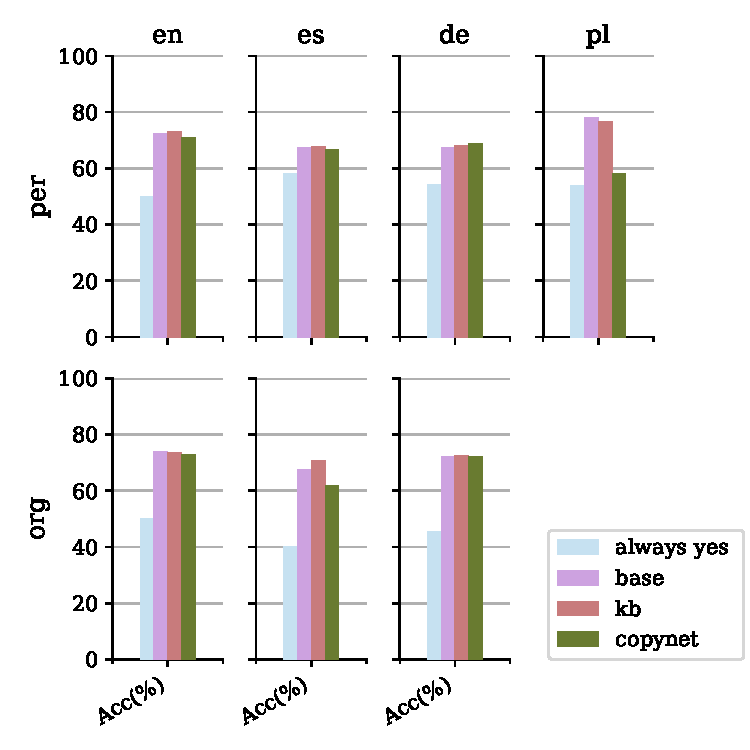
\includegraphics{yes-no_gold_results.pdf}}
    \caption{}
    \end{subfigure}
    \begin{subfigure}{0.59\linewidth}
    \resizebox{\textwidth}{!}{
    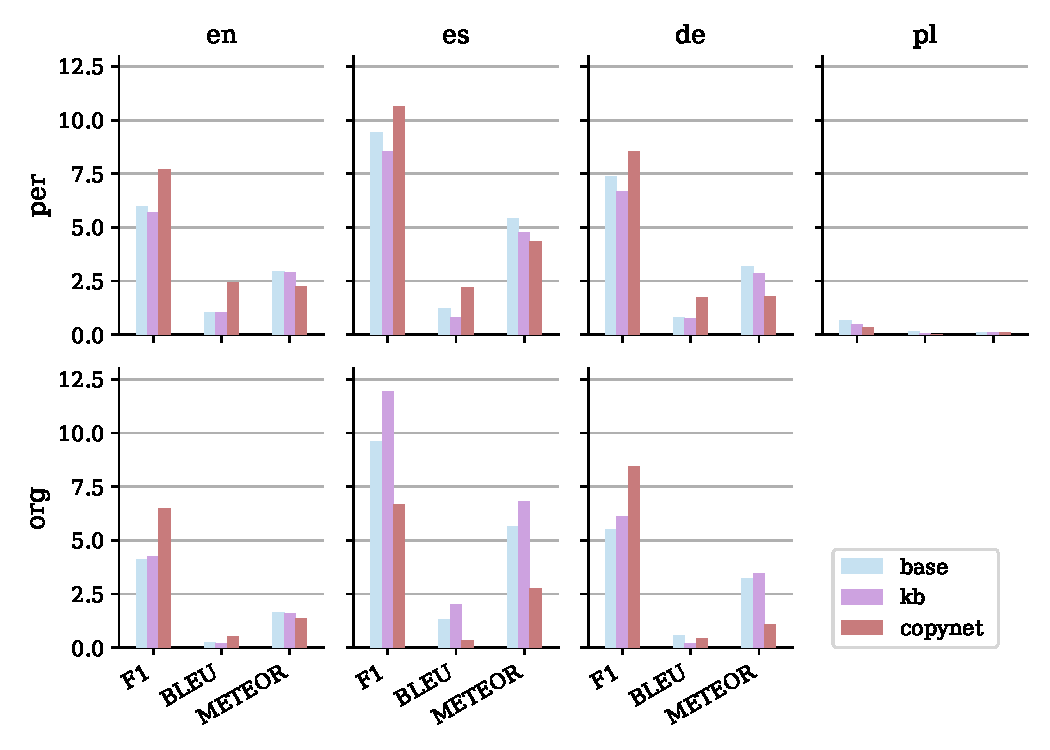
\includegraphics{generation_gold_results.pdf}}
    \caption{}
    \end{subfigure}
    \caption{(a) Evaluation of (a) the models' ability to correctly decide when an appositive is due, (b) generated predictions for positive test instances. Measured on the News test set. }
    \label{fig:gold}
\end{figure*}

The full range of results on the News test set are shown in Figure~\ref{fig:gold}. Results are averaged over three models trained from different random initializations. We evaluate how well the models can detect when an appositive is needed (implicit classification) and how well it can perform the end-to-end task of classifying and generating a good appositive.

\paragraph{Implicit classification} of the positive and negative samples in the data appears to be roughly equally challenging across the two entity types and the four languages, as viewed across all three models (see Figure~\ref{fig:gold}a. One exception is Polish \textsc{person} appositives, where \texttt{base} and \texttt{kb} score higher than they do on the other subsets, while \texttt{copynet} barely beats the baseline. Since the models are not explicitly trained to perform this type of classification, it is encouraging to see that even in this setting, they can outperform the baseline (always predicting the positive class) by as much as 20\% in several cases.

\paragraph{Generation} is the more difficult aspect of the task, as shown in Figure~\ref{fig:gold}b. We see that, somewhat surprisingly considering the amounts of training data (see Table~\ref{tab:silver_data_stats}),  performance is not highest on English, but rather on Spanish. In line with the small amount of training data, on the other hand, performance on Polish is virtually non-existent. There are no clear differences between overall performance on \textsc{person} and \textsc{organization} appositives. Only in English, the latter seem to pose a greater challenge to all three models and according to all three metrics. Model comparison is not straightforward since the different metrics reveal different strengths and weaknesses in each approach. It does appear to be the case that injecting external knowledge through pretrained knowledge-base embeddings (\texttt{kb}) is beneficial to the prediction of \textsc{organization} appositives and somewhat harmful to the prediction of \textsc{person} appositives. Since the differences between the three methods are not consistent across all languages, named entity types and metrics, we cannot conclusively say which method is best, but we do note that \texttt{copynet} scores high on the most metrics, languages and entity types. To better understand the performance of this model, we stepped away from automatic generation metrics, which are known to suffer from certain biases and can be difficult to interpret, and we carried out an additional manual evaluation.%\jttodo{I like this segue}
%In the analysis presented below, we therefore focus on the predictions of this model.  
%\jttodo{we should qualify why these numbers look low.  Maybe mention the Kang paper?  Or just the limitations of the metrics for this task?  How did Kang hedge things?}  
%\jttodo{In fact (coming back to this section) we could say that the limitations of the metrics (and maybe other things) motivated the use of human evaluation to definitively evaluate our top method and to get a sense of how well a system can really predict and generate an appos.  Also note that this is the first time someone is doing this comparison.  (and yes first time out of two papers haha).  Anyway, that acknowledges limitations of an automatic eval while setting us up for Sec 7.   }

\section{Analysis}
\label{sec:analysis}
\subsection{Manual evaluation}
We used Amazon Mechanical Turk to carry out a ranking paradigm study on the predictions of \texttt{copynet} for English \textsc{person} and \textsc{organization} appositives. The annotators were shown a true appositive and a predicted appositive side-by-side (in the context of the input sentence) and were asked to express their preference towards either of these two, or their lack of preference as a third option. One example prompt is shown in Appendix~\ref{taste_test}. Five annotations were obtained per data instance, and we then took the majority vote as an indication of the overall preference. %\jttodo{we don't have space to put these numbers in a table?  It would just look nicer and would be easier to follow}
The results are shown in Table \ref{tab:manual_eval}.  
For  \textsc{person} appositives, the writer's choice (true) and the system's prediction 
%True and predicted \textsc{person} appositives 
were preferred at almost equal rates---this observation challenges the numbers obtained with the automatic evaluation metrics, as it suggests that the predicted appositives were not necessarily of poor quality. A bigger gap was observed between true and system-generated \textsc{organization} appositives, where the crowdworkers preferred the original appositive 66.0\% of the time. The lower preference for \textsc{organization} predictions is in line with the trend in the automatic results, where performance on English \textsc{organization} appositives was shown to be lower than that on English \textsc{person} appositives.  Notice, however, that even for \texttt{organization} appositives, annotators still showed preference for the predicted ones at a considerable rate. This suggests that the automatic metrics may have severely under-represented the abilities of the models. 

%The rate of neutrality was low for both entity types. 


\begin{table}[]
    \centering
    \small
    \begin{tabular}{llllllll}
         & true & system & neutral && true & system & neutral \\
         \textsc{per}& 46.3\% & 47.3\% & 6.1\%  & \textsc{org}& 66.0\% & 26.5\% & 7.4\% \\
         
    \end{tabular}
   \caption{Results from the ranking paradigm study comparing true appositives to system-generated ones.}
    \label{tab:manual_eval}
\end{table}


\subsection{Qualitative analysis}
To better understand the source of error in the models' predictions, we manually inspected 50 data points from  the \textsc{person} subset and 50 data points from the \textsc{organization} subset, where a choice was made in favour of the true appositive over the predicted one. Half of the data points were instances where the true appositive was not empty, but the models predicted an empty appositive. The annotators seemed to strongly prefer non-empty appositives, possibly due to the fact that they where shown sentences without their original context, where the role of an entity might have been clarified at an earlier mention. Yet, that is not categorically so as seen in example 1 in Table~\ref{tab:examples}, where the predicted appositive is redundant in the given context, so the annotators preferred the true empty appositive. Other types of errors the models made were to predict appositives that concern the right piece of information but are too general (examples 2 and 3), to predict appositives based on the wrong piece of information (examples 4 and 5), and, specifically for \textsc{organization} appositives, to just repeat the named entity (example 6).   While the latter is the result of either suboptimal learning or noise in the data, the rest of the errors we saw point to the need for an approach with deeper understanding of the facts and their relevance to the context.

% left fixed width:
\newcolumntype{L}[1]{>{\raggedright\arraybackslash}p{#1}}
% center fixed width:
\newcolumntype{C}[1]{>{\centering\arraybackslash}p{#1}}
% flush right fixed width:
\newcolumntype{R}[1]{>{\raggedleft\arraybackslash}p{#1}}
\begin{table*}[]
    \small
    \resizebox{\textwidth}{!}{
    \begin{tabular}{L{0.005cm}L{11.7cm}L{2.9cm}}
        &Gold sentence & Prediction \\
        \hline
        1&In response to an April 9 court ruling declaring the military backed government of Frank Bainimarama \textcolor{blue}{\texttt{<EMPTY>}} to power illegally when he dissolved Parliament and deposed the government of Laisenia Qarase , the country ’s President nullified the Fiji 's constitution , fired the entire judiciary and appointment himself head of state and the armed forces. & the President of Fiji\\
        2&Artyom Loskutov, \textcolor{blue}{creator of the popular counter - culture art movement " Monstration "}, made waves on RuNet by signing a letter in support of Dmitry Kiselyov , a journalist who many consider to be Putin 's chief propagandist. & a Russian painter\\
        3&In a fatal blow to our already lackluster sources of entertainment , the Sudanese government has blocked access to YouTube,  \textcolor{blue}{the online video sharing Web site}. & platform \\
        3&Modi, \textcolor{blue}{a tech-savvy nationalist from the right-wing Bharata Janatiya Party}, has traveled the world to sell the idea of India as an emerging digital economy, making deals with the likes of Google and ( less successfully ) Facebook. & the Prime minister of India \\
        4&Some critics also highlighted the fact that Jabrailov is from Chechnya, \textcolor{blue}{a republic in the Northern Caucasus region of Russia where Muslim separatists fought two bloody wars against the Russian army}.&Chechnya\\
        5&He steers between Soukous , rhumba and RnB ” , and links to an interview with the singer on Radio Okapi,  \textcolor{blue}{the nationwide radio station sponsored by the UN and Fondation Hirondelle}. & the Democratic Republic of the Congo\\
        6&In particular , tweeps took note of Abed Rabbo 's attacks on Qatar, \textcolor{blue}{the home of Al Jazeera}. & Qatar\\
    \end{tabular}
    }
    \caption{Examples where true appositives were preferred over predicted ones by human annotators.}
    \label{tab:examples}
\end{table*}


\section{Conclusion}
\label{sec:conclusion}
\corpus~ targets factual appositive generation, a phenomenon frequently occurring in a range of textual domains.  It substantially extends the prior resources in the area by spanning four languages, two named entity types 
%(\textsc{person} and \textsc{organization})
, and two domains.  This resource also allows the burgeoning field to investigate end-to-end appositive generation.  
%Spanning four languages, it allowed us to uncover some surprising findings---that more data does not always lead to better performance on this task (compare English to Spanish), and also some expected ones---that limited data leads to rather poor performance (Polish). 
%Spanning four languages, the dataset also covers two named entity types, \textsc{person} and \textsc{organization}, which in terms of automatic metrics appeared to be handled similarly by the our models. 
Our manual and automatic evaluations with \corpus~ show that standard model architectures can approach the quality of human targets in specific cases but there is still room for improvement.
%??? 
%But human evaluation revealed that the latter subset is indeed substantially harder to model than the former. 
With this dataset, appositive generation can be studied in much more depth than previously possible, ultimately paving the way for novel NLP applications in the generation and writing space. The focus in future research, we believe, should fall on explicit methods for cross-domain learning, on richer knowledge sources, and on the development of test sets for new domains. 

\section{Acknowledgements}
We acknowledge the responsiveness and help of Jun Seok Kang and Robert L. Logan IV in discussions on the design choices and goals of their work on post-modifier generation and on how to accurately reproduce their experiments.  We also thank researchers from Dataminr: Saran Krishnasamy, Lin Nie, and Isabel Zhang for their help in setting up experiments and annotation.  Finally, we thank the three anonymous reviewers for their feedback and comments.

%two DEs gave feedback on MTurk.  Lin Nie and Isabel Zhang.  DEs

%\jttodo{we need an acknowledgments section; totally ack Kang and his co-authors, and anyone (in DM or outside) that helped run code.  } \yktodo{Joel, feel free to add anyone else, e.g. the person who was setting up GPUs for me at DM? Unfortunately, I have forgotten his name and can no longer retrieve it from Slack/email.I feel like he deserved a big thank you.}

%\jttodo{my comments from before (see below) still stand.  Sell the work :)}
%\jttodo{I'm leaving this alone until the end.  But can you include some text around:  1) remind the reader how we expand the task formulation and create a new dataset really to bring the task closer to a real-world setting.  2) future work into how this dataset could be further expanded  3) future work into modeling - what approaches could be tried, the effect of new databases, etc.  and perhaps why Kang's set would not be able to achieve that.  What I'm going for here is to say this is the second paper in this area but it really opens up the field.}

%\section{Alternate Conclusion}
%\label{sec:conclusion2}

%News articles, image captions, product reviews and many other texts mention people and organizations whose name recognition could vary for different audiences. In such cases, background information about the named entities could be provided in the form of an appositive noun phrase, either written by a human or generated automatically.
%We expand on the previous work in appositive generation with a new, more realistic, end-to-end definition of the task, instantiated by a dataset that spans four languages (English, Spanish, German and Polish), two entity types (person and organization) and two domains (Wikipedia and News). 
%We carry out an extensive analysis of the data and the task, pointing to the various modeling challenges it poses. The results we obtain with standard language generation methods show that the task is indeed non-trivial, and leaves plenty of room for improvement.  

%\jttodo{other stuff: subjective appos generation}

%The dataset we introduce targets a phenomenon frequently occurring in News articles and as such could be used in the development of writing assistants for the News domain. In more general terms, appositive generation lies at the interface of language understanding and language generation, proving to be an interesting NLP task in itself. Our preliminary results show that the NLU aspect of the problem is indeed the more challenging one. Methods that rely on explicit reasoning over external knowledge resources could therefore likely yield substantial improvements. Moreover, the cross-domain nature of the data makes it a suitable test bed for methods for domain transfer.   


\bibliographystyle{coling}
\bibliography{coling2020}

\clearpage
\appendix

\section{Appendices}

\subsection{Manual validation} 
\label{manual}
We hired annotators fluent in the languages of the data to manually validate it. They had to mark instances where an error had occurred in the appositive detection, the detected appositive was not factual, or the entity had been incorrectly linked to WikiData (all instances of \textit{noise} in the data, resulting from errors in appositive detection and entity linking). Our ultimate goal was to build test sets of 1,000 instances per language per entity type, equally balanced between positive and negative instances, i.e. we needed 500 valid data instances per language per entity type. Based on a pilot study, we determined that noise levels for candidate appositives for \textsc{person} entities were approximately 33\% and for \textsc{organization} entities, 50\% (averaged across languages). We therefore gave annotators 750 and 1,000 candidates to annotate for the \textsc{person} and \textsc{organization} types, respectively. For most language-entity type combinations, the manual annotation successfully yielded close to 500 valid instances. That was not the case for Polish \textsc{organization} appositives, where only 80 valid candidates were retrieved, so we excluded this language-entity type combination from our work. It remains an open question whether \textsc{organization} appositives in Polish are rare or our automatic detection method failed at catching them. 

\subsection{Composition of cross-lingual data}
\label{composition}
Table~\ref{tab:facttypes} present findings on the composition of the Spanish, German and Polish positions of the data, respectively, as observed through cross-referencing with WikiData. The low number of facts for Polish is the result of one fact type dominating a large amount of the data (\textit{position held}).

\begin{table}[]
    \begin{subtable}{0.45\textwidth}
    \centering
    \small
    \begin{tabular}{clll}
                         &Fact type&News (\%)&Wiki(\%)\\
                         \hline                         %\multirow{10}{*}{\rotatebox{90}{\textsc{org-entity}}}&sovereign state&sovereign state\\
                         %&country&country\\
                         %&business&business\\
                         %&organization&big city\\
                         %&big city&\textcolor{gray}{enterprise}\\
                         %&political party&city\\
                         %&city&city 1000000+\\
                         %&city of the USA&political party\\
                         %&city 1000000+&\textcolor{gray}{capital}\\
                         %&university&\textcolor{gray}{landlocked country}\\
                         %\hline                         
                         \multirow{7}{*}{\rotatebox{90}{\textsc{per}}}&  position held & 20.9 & 9.4 \\ 
                          & occupation&15.9&10.6\\
                          & citizenship&10.1&4.3\\
                          & member of party&7.6&1.9\\
                          & award received&5.2&3.9\\
                          & nominated for&3.6&0.4\\
                          & educated at&3.1&3.1\\
                         \hline
                         \multirow{7}{*}{\rotatebox{90}{\textsc{org}}} & instance of&23.1&10.9\\
                         & official website & 6.3&6.2\\
                         & country&5.9&3.3\\
                         & member of&4.2&2.4\\
                         & subsidiary&3.5&2.1\\
                         & capital of&3.2&0.1\\
                         & has quality&3.0&0.0\\
    \end{tabular}
    \caption{English }
    \label{tab:wikidata_en}
    \end{subtable}
    \begin{subtable}{0.45\textwidth}
    \small
    \centering
    \begin{tabular}{clll}
                         &Fact type&News (\%)&Wiki(\%)\\
                         \hline                       \multirow{7}{*}{\rotatebox{90}{\textsc{per}}}&  position held&27.1&4.9\\
                          & occupation&11.2&10.3\\ 
                          & citizenship&9.8&4.8\\
                          & participant of&8.7&1.1\\
                          & member of party&7.3&1.3\\
                          & award received&4.1&3.2\\
                          & employer&3.2&0.5\\
                         \hline \multirow{6}{*}{\rotatebox{90}{\textsc{org}}} & instance of&28.9&10.5\\
                         & country&7.8&3.5\\
                         & has quality&5.1&0.1\\
                         & capital of&4.4&0.5\\
                         & member of&4.3&2.9\\
                         & is located in&3.4&2.2\\
    \end{tabular}
    \caption{Spanish }
    \label{Spanish}
    \end{subtable}
    \begin{subtable}{0.45\textwidth}
    \small
    \centering
    \begin{tabular}{clll}
                         &Fact type&News (\%)&Wiki(\%)\\
                         \hline                       \multirow{8}{*}{\rotatebox{90}{\textsc{per}}}&  position held&35.2&6.7\\
                          & employer&5.9&2.9\\ 
                          & citizenship&5.9&1.3\\
                          & member of party&5.3&2.4\\
                          & award received&4.9&2.1\\
                          & occupation&4.8&3.6\\
                          & participant of&4.6&1.5\\
                          & member of & 3.6&1.0\\
                         \hline \multirow{6}{*}{\rotatebox{90}{\textsc{org}}} & official website&15.6&12.4\\
                         & instance of&15.1&4.5\\
                         & owner of&7.5&2.4\\
                         & member of&5.8&0.9\\
                         & has quality&4.6&0.0\\
                         & Commons category&3.2&4.5\\
    \end{tabular}
    \caption{German }
    \label{German}
    \end{subtable}
    \begin{subtable}{0.45\textwidth}
    \small
    \centering
    \begin{tabular}{clll}
                         &Fact type&News (\%)&Wiki(\%)\\
                         \hline                       \multirow{2}{*}{\rotatebox{90}{\textsc{per}}}&  position held&77.2&5.7\\
                          & participant of&3.2&0.7\\

    \end{tabular}
    \caption{Polish }
    \label{Polish}
    \end{subtable}
    \caption{Top fact types per language.}
    \label{tab:facttypes}
\end{table}

\subsection{Implementations and hyperparameters}
\label{implementation}
\paragraph{[Base] and [KB]}
We use the implementation of \newcite{kang2019pomo} from \url{https://github.com/rloganiv/claimrank-allennlp}. We set the model hyperparameters to the ones reported in their paper, changing only the dimension of the embeddings from 500 to 300, to make the comparison between [Base] and [KB] fair in terms of model parameterization. Training hyperparameters were tweaked to achieve stable training that fits on one 16 GB GPU. See the full list of hyperparameters in Table~\ref{tab:hps}.

\subsection{Projection of NTEE embeddings}
\label{projection}
We obtained a bilingual dictionary with CSLS retrieval over the cross-lingual FastText embeddings. CSLS retrieval is similar to nearest neighbor retrieval, but has proven more accurate: \cite{joulin-etal-2018-loss} report an accuracy of 83.7\%, 77.6\% and 73.5\% for word translation, respectively, from Spanish, German and Polish to English, as measured on a sample of 1,500 medium frequency words. Any errors in the bilingual dictionaries would inevitably lead to noise in the NTEE embedding projection.

\paragraph{Copynet}
We use the AllenNLP \cite{Gardner2017AllenNLP} implementation of Copynet with the hyperpameters shown in  Table~\ref{tab:hps}.

\begin{table}[]
    \centering
    \small
    \begin{tabular}{lll}
         &  Base/KB & Copynet \\
         \hline
         vocab size & 50k & 50k \\
         embedding dim & 300 & 300 \\
         hidden units & 250 & 250 \\
         num layers & 2 & 2 \\
         optimizer & Adam & Adam \\
         learning rate & 0.001 & 0.0001 \\
         batch size & 16 & 6 \\
         dropout & 0.3 & 0.3 \\

    \end{tabular}
    \caption{Hyperparameter configurations for Base/KB models and Copynet models.}
    \label{tab:hps}
\end{table}

\subsection{Transformer experiments}
\label{transformer}
%\paragraph{Transformer}\jttodo{Given space constraints I say we move this to the appendix.  But we turn it into a footnote and attach it to my new sentence in the beginning of Sec 6 where I state that the goal is not to make the best model }
Transformer-based architectures are state-of-the-art for many NLP tasks, so it is only fair that we experiment with such an architecture as well. As BERT models \cite{devlin2019bert} have been made available for all four languages we work with, we chose to train BERT-to-BERT encoder-decoder models for appositive generation. \newcite{DBLP:journals/corr/abs-1907-12461} found that architecture to give strong performance on tasks like sentence fusion and rephrasing. We used their training schedule but unfortunately, found that all models learned to predict the \texttt{<empty>} token exclusively. As it is not the goal of our work to explore the capabilities of the BERT-to-BERT architecture in particular, we did not use further resources to adjust the training schedule. Yet, we do believe this to be an optimization problem, and we would not discourage future research from attempting to solve the task of appositive generation with a transformer-based approach.
%\jttodo{to come back to: let's see how the paper comes together.  We may want to shrink this down but explain things more fully in an Appendix.}




\subsection{Results}
The results as measured on the Wikipedia test set are shown in Figure~\ref{fig:silver}. Compared to results on the News test set (see Figure~\ref{fig:gold}, the numbers seen here are higher, which is to be expected considering that this test set is in-domain and any noise found in it (due to it being silver standard) likely resembles the noise found in the training data. It is worth noting though, that certain patterns repeat between the two test sets, as for example the fact that \texttt{copynet}, as measured on F1 score and BLEU, outperforms the other models on the majority of language-named entity type combinations, but not on Polish \textsc{person} appositives and Spanish \textsc{organization} appositives. This suggests that, while evaluation on the silver-standard Wikipedia test set cannot be consider fully stable and representative, it can be taken as a proxy in model comparison for developmental purposes.
\begin{figure*}
    \centering

    \begin{subfigure}{0.39\linewidth}
    \resizebox{\linewidth}{!}{
    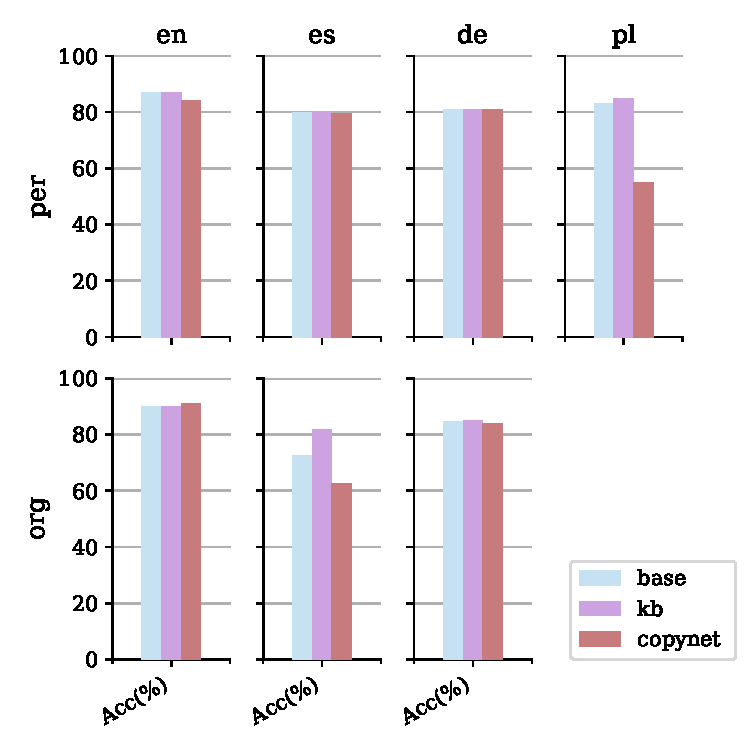
\includegraphics{yes-no_silver_results.pdf}}
    \caption{}
    \end{subfigure}
    \begin{subfigure}{0.59\linewidth}
    \resizebox{\textwidth}{!}{
    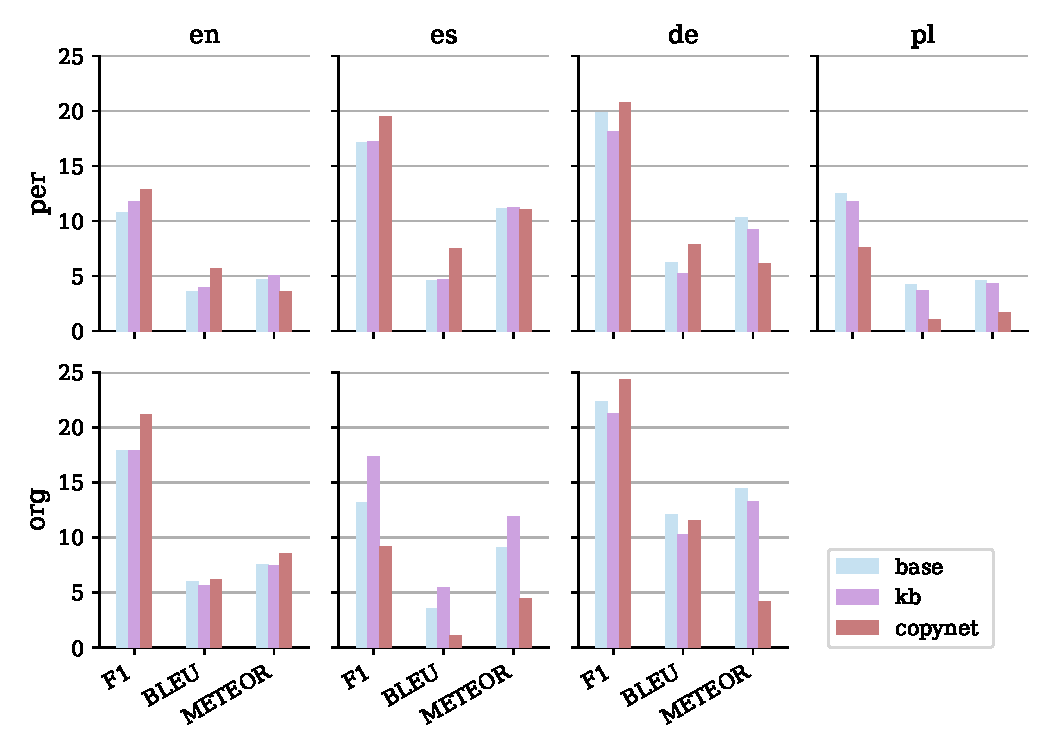
\includegraphics{generation_silver_results.pdf}}
    \caption{}
    \end{subfigure}
    \caption{(a) Evaluation of (a) the models' ability to correctly decide when an appositive is due, (b) generated predictions for positive test instances. Measured on the News test set. }
    \label{fig:silver}
\end{figure*}

The numbers behind the results from Figures~\ref{fig:gold} and~\ref{fig:silver} are shown in Tables~\ref{tab:gold_results} and ~\ref{tab:silver_results}, respectively.

\begin{table*}[]
    \centering
    \begin{tabular}{cllllllll}
        && Acc & F1 & BLEU & METEOR\\
        \hline
        \multirow{3}{*}{\rotatebox{90}{\textsc{en-per}}}&always yes &0.5&0.0&0.0&0.0\\
        &base &71.91&0.72&1.03&2.96\\
        &kb &71.73&0.73&1.03&2.9\\
        &copynet &70.19&0.71&2.45&2.24\\
        \hline
        \multirow{3}{*}{\rotatebox{90}{\textsc{en-org}}}&always yes &0.5&0.0&0.0&0.0\\
        &base &68.09&0.74&0.23&1.61\\
        &kb &66.58&0.74&0.21&1.58\\
        &copynet &65.98&0.73&0.52&1.37\\
        \hline
        \multirow{3}{*}{\rotatebox{90}{\textsc{es-per}}}&always yes &0.58&0.0&0.0&0.0\\
        &base &62.84&0.67&1.24&5.44\\
        &kb &61.18&0.68&0.79&4.79\\
        &copynet &64.08&0.67&2.2&4.36\\
        \hline
        \multirow{3}{*}{\rotatebox{90}{\textsc{es-org}}}&always yes &0.4&0.0&0.0&0.0\\
        &base &47.39&0.68&1.32&5.64\\
        &kb &60.91&0.71&2.02&6.83\\
        &copynet &33.57&0.62&0.33&2.77\\
        \hline
        \multirow{3}{*}{\rotatebox{90}{\textsc{de-per}}}&always yes &0.54&0.0&0.0&0.0\\
        &base &62.94&0.67&0.8&3.19\\
        &kb &63.47&0.68&0.75&2.84\\
        &copynet &67.63&0.69&1.75&1.76\\
        \hline
        \multirow{3}{*}{\rotatebox{90}{\textsc{de-org}}}&always yes &0.46&0.0&0.0&0.0\\
        &base &62.77&0.72&0.54&3.21\\
        &kb &65.13&0.73&0.19&3.47\\
        &copynet &62.22&0.72&0.43&1.08\\
        \hline
        \multirow{3}{*}{\rotatebox{90}{\textsc{pl-per}}}&always yes &0.54&0.0&0.0&0.0\\
        &base &72.83&0.78&0.16&0.09\\
        &kb &73.8&0.77&0.06&0.13\\
        &copynet &2.75&0.58&0.0&0.12\\
    \end{tabular}
    \caption{Evaluation of the models' ability to correctly decide when an appositive is due and of generated predictions for positive test instances. Measured on the News test set. }
    \label{tab:gold_results}
\end{table*}

\begin{table*}[]
    \centering
    \begin{tabular}{cllllllll}
    \hline
    \multirow{3}{*}{\rotatebox{90}{\textsc{en-per}}}&base &85.42&0.87&3.59&4.7\\
    &kb &85.32&0.87&3.94&5.07\\
    &copynet &81.95&0.84&5.7&3.57\\
    \hline
    \multirow{3}{*}{\rotatebox{90}{\textsc{en-org}}}&base &89.47&0.9&5.99&7.54\\
    &kb &89.43&0.9&5.65&7.49\\
    &copynet &89.17&0.91&6.17&8.53\\
    \hline
    \multirow{3}{*}{\rotatebox{90}{\textsc{es-per}}}&base &78.49&0.8&4.57&11.17\\
    &kb &78.73&0.8&4.71&11.19\\
    &copynet &79.1&0.8&7.54&11.04\\
    \hline
    \multirow{3}{*}{\rotatebox{90}{\textsc{es-org}}}&base &61.63&0.73&3.58&9.07\\
    &kb &80.69&0.82&5.45&11.92\\
    &copynet &46.91&0.62&1.14&4.46\\
    \hline
    \multirow{3}{*}{\rotatebox{90}{\textsc{de-per}}}&base &79.28&0.81&6.19&10.35\\
    &kb &80.09&0.81&5.24&9.19\\
    &copynet &80.12&0.81&7.85&6.11\\
    \hline
    \multirow{3}{*}{\rotatebox{90}{\textsc{de-org}}}&base &84.09&0.85&12.04&14.45\\
    &kb &84.58&0.85&10.28&13.31\\
    &copynet &82.07&0.84&11.57&4.19\\
    \hline
    \multirow{3}{*}{\rotatebox{90}{\textsc{pl-per}}}&base &82.67&0.83&4.23&4.61\\
    &kb &84.46&0.85&3.67&4.29\\
    &copynet &24.49&0.55&1.1&1.71\\
    \end{tabular}
    \caption{Evaluation of the models' ability to correctly decide when an appositive is due and of generated predictions for positive test instances. Measured on the Wiki test set. }
    \label{tab:silver_results}
\end{table*}

\subsection{Ranking paradigm study}
\label{taste_test}
Figure~\ref{fig:tastetest} shows an example prompt from the blind taste test. Instances where either the true appositive was empty or the predicted one was empty were included in the the study, but instances where both were empty were excluded, as the comparison would not have been meaningful in this case. The average time for completing a HIT was 53 seconds.
\begin{figure}
    \centering
    \resizebox{0.55\linewidth}{!}{
    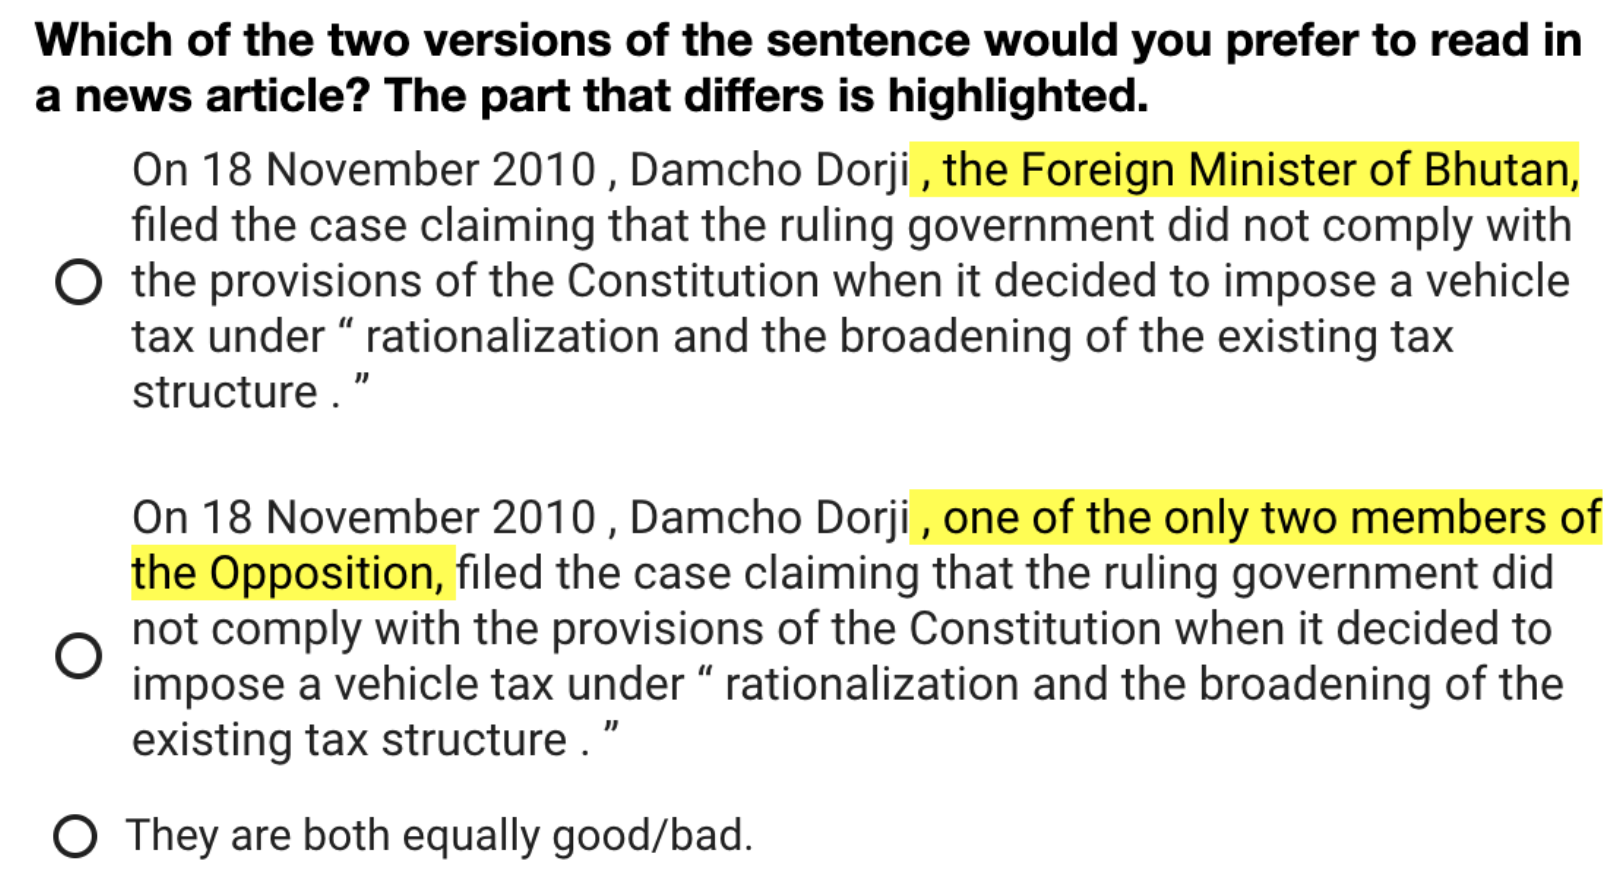
\includegraphics{tastetest.png}}
    \caption{Prompt for manual evaluation.}
    \label{fig:tastetest}
\end{figure}

\end{document}
